\hspace*{12pt}Los resultados obtenidos para la luminosidad de cada estrella en la vecindad solar son los que siguen:

	\begin{figure}[!htbp]
		\centering
		\title{\textbf{Histograma de luminosidades}}
		\begin{center}
			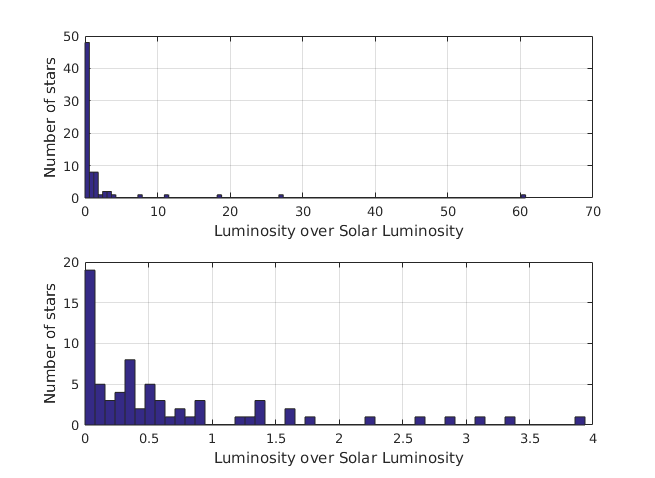
\includegraphics[width=15cm]{Figures/Lhist.png}
		\end{center}
		\caption{\footnotesize{
		Distribuci\'{o}n obtenida para la muestra. En la \textit{Figura 1.1} (Arriba) se muestra el n\'{u}mero de estrellas con una determinada luminosidad comparada con la luminosidad del Sol. En la \textit{Figura 1.2} (Abajo) se ha representado el mismo gr\'{a}fico para el subconjunto muestral mayoritario, el cual se distribuye alrededor de la luminosidad del sol.}}
		\label{Lhist}
	\end{figure}

	Como se puede observar en la Figura \ref{Lhist}, la gran mayor\'{i}a de las estrellas en la vecindad solar emiten con una luminosidad menor a la del Sol. En concreto, m\'{a}s del 50\% de las estrellas presentan una luminosidad menor que la mitad de la luminosidad solar. M\'{a}s adelante, en la Figura \ref{HRdiag}, se explica c\'{o}mo esto est\'{a} relacionado la selecci\'{o}n de estrellas restingida en los tipos espectrales A, F, G y K y el tiempo de vida media caracter\'{i}stico de cada tipo espectral.